\def\year{2016}
%File: formatting-instruction.tex
\documentclass[letterpaper]{article}
\usepackage[ruled,vlined,linesnumbered]{algorithm2e}
\usepackage{aaai}
\usepackage{times}
\usepackage{helvet}
\usepackage{color}
\usepackage{graphicx}
\usepackage{courier}
\usepackage{amsthm}
\usepackage{amsmath}
\usepackage{url}

\newcommand\note[1]{\textcolor{red}{#1}}

\frenchspacing
\setlength{\pdfpagewidth}{8.5in}
\setlength{\pdfpageheight}{11in}



\pdfinfo{
/Title (Stronger Privacy Preserving Projections for Multi-Agent Planning)
/Author (Submission \#761)}
\setcounter{secnumdepth}{0}  

\newtheorem{definition}{Definition}
\newtheorem{theorem}{Theorem}
\newcommand\roni[1]{\textcolor{blue}{roni: #1}}
\newcommand\guy[1]{\textcolor{red}{guy: #1}}

\theoremstyle{definition}
\newtheorem{example}{Example}[section]


\setcounter{secnumdepth}{2}

 \begin{document}
% The file aaai.sty is the style file for AAAI Press 
% proceedings, working notes, and technical reports.
%
\title{Stronger Privacy Preserving Projections for Multi-Agent Planning}
\author{Submission \#761}
%\author{Shlomi Maliah \and Guy Shani \and Roni Stern \\
%Association for the Advancement of Artificial Intelligence\\
%2275 East Bayshore Road, Suite 160\\
%Palo Alto, California 94303\\
%}
\maketitle
\begin{abstract}
\begin{quote}
Collaborative privacy-preserving planning (CPPP) is a multi-agent planning task in which agents need to achieve a common set of goals without revealing certain private information to each other. In many privacy-aware planning algorithms the individual agents reason about a {\em projection} of the multi-agent problem onto a single agent classical planning problem. 
For example, an agent can behave as if it controls the public actions of other agents, ignoring their unknown private preconditions and effects. This projection, however, contains very minimal information, ignoring the dependencies between public actions of other agents. We propose a stronger type of projection, in which the information about the dependencies between the public actions is published to all agents. In addition, we propose a new definition of privacy referring to the number of private facts or objects an agent controls, and show that we do not disclose such information.
%We demonstrate the benefits of our stronger projection, showing that it produces high level plans very fast, solving more benchmark problems than any other state-of-the-art privacy preserving planners. 
The benefits of our stronger projection are demonstrated by showing that it produces high level plans very fast, solving more benchmark problems than any other state-of-the-art privacy preserving planners. 
%Privacy-aware planning algorithm are orders of magnitude slower than existing single agent planners that ignore privacy. We propose a method for projecting a privacy-preserving planning problem to a single agent planning problem without compromising privacy. A solution to the resulting planning problem can in most cases be trivially extended to be a solution to the original privacy preserving problem. The resulting privacy-preserving planner is shown to compare favorably with state-of-the-art privacy preserving planners. 
\end{quote}
\end{abstract}


\section{Introduction}


%Designing autonomous agents able to act collaboratively as a team is a long standing goal in Artificial Intelligence. A fundamental aspect of such collaboration is the ability to plan for multiple agents acting in the world. In this work we address the problem of planning for multiple agents 

% What is CPPP and why we care
{\em Collaborative privacy preserving planning (CPPP)} is a multi-agent planning task in which agents need to achieve a common set of goals without revealing certain private information. CPPP has important motivating examples such as planning for organizations that outsource some of their tasks and collaboration between military units where compartmentalization is required. CPPP recently received much attention~\cite{brafman2013complexity,nissim2014distributed,Brafman15,torreno2014aFlexible,maliah2014privacyPreserving,torreno2014fmap,torreno2015global,tovzivcka2014generating,jakubuv2015multiagent} and new efficient solvers, scaling up to larger, more challenging domains are constantly proposed.
%\roni{This is very compressed and can be extended and improved}

% CPPP is nice, by single agent planning is much faster
%Even though research on CPPP is flourishing, classical planning algorithms are substantially more mature, offering very fast solvers with strong heuristics \cite{hoffmann2001ff,helmert2009landmarks}. An attractive approach, hence, is to {\em project} the multi-agent privacy preserving problem onto a classical planning problem, and employ a classical solver. Some planners use the resulting plan as a high-level plan for the individual agents to extend~\cite{tovzivcka2014generating,jakubuv2015multiagent,maliah2014privacyPreserving}, while other planners use the cost of that plan as a heuristic~\cite{nissim2014distributed}.

% view and projection
%Due to privacy, each individual agent has only a partial view of the world, containing its own private facts and actions, and its public actions. The agent also knows about the public actions of other agents, but is aware only of their public preconditions and effects. One can treat the agent view of the world as a classical planning problem, pretending that the agent controls the public actions of others. Then, one could solve this classical projection and obtain a plan.\roni{This repeats the above so I merged them}

% CPPP is nice, by single agent planning is much faster
Even though research on CPPP is flourishing, classical planning algorithms are substantially more mature, offering very fast solvers with strong heuristics \cite{hoffmann2001ff,helmert2009landmarks}. An attractive approach, hence, is to {\em project} the multi-agent problem onto a classical planning problem,  employ a classical solver, and then extend the resulting public plan using private actions. 
%Some planners use the resulting plan as a high-level plan for the individual agents to extend~\cite{tovzivcka2014generating,jakubuv2015multiagent,maliah2014privacyPreserving}, while other planners use the cost of that plan as a heuristic~\cite{nissim2014distributed}.

% view and projection
Due to privacy, each individual agent has only a partial view of the world, containing its own public and private facts and actions. The agent also knows about the public actions of other agents, but is aware only of their public preconditions and effects. One can treat the agent view of the world as a classical planning problem, pretending that the agent controls the public actions of others. Then, one could solve this classical projection and obtain a plan.

%this projection is less than great
In this single-agent projection of the multi-agent world, the agent is unaware of internal dependencies between other agents' public actions. This results in an over optimistic assumption about what other agents can do. For example, in a blocksworld domain, where each agent controls a different arm, and the blocks held by an arm are private information, a an action that puts block $A$ on top of block $B$ does not publish the private precondition for holding the $A$ to begin with. Hence, the other agents may believe that the $A$ can be put everywhere without picking it up.


% Without a good projection, we need to synchronize, which sucks
As a solution to this single-agent projection is not necessarily a sound solution to the mulit-agent planning, some mechanism is required to publish additional information required for constructing a sound plan. For example, in the MAFS algorithm~\cite{nissim2014distributed} agents broadcast partially encrypted states to all agents whenever a public action is performed. In the PSM algorithm~\cite{tovzivcka2014generating} agents continuously generate and share single-agent plans until a valid combination of single agent plans is reached. Methods of this type use a  multi agent planning mechanism, where all agents plan together, jointly revealing additional important information.

In this paper we take a different approach. We suggest a stronger projection, where all agents publish a projection of their private view of the world, containing only public actions. The joint single agents projections is fed into a classical planner, resulting in a high level plan for achieving the goals, constructed only of public actions~\cite{maliah2014privacyPreserving}. Then, each agent extends the plan by adding private actions that allow it to perform its part in the public plan~\cite{tozicak2015onInternally}. 

% Our approach: share the internal dependencies
As the main lack of required information in the simple projection is the lack of dependencies between the public actions of an agent, we focus on identifying these dependencies. We define new facts that represent these dependencies, and explain when to add, and when to delete these dependency facts. The usefulness of the proposed projection is demonstrated in practice in a simple planner that uses a solution of the projected problem as a skelton plan that is extended by all agents. The resulting planner solves more benchmarks from the distributed multi-agent competition (CoDMAP)~\cite{vstolba2015competition} than any other state-of-the-art privacy preserving planner. 

% But what about privacy??

In addition, we discuss a new definition of privacy which we call {\em cardinality-hiding privacy}. In many domains agents are interested in hiding from other agents the number of private facts or objects. For example, a logistic company may wish to hide the number of trucks it controls, and the military would not disclose the number of bases in an area. An algorithm is {\em cardinality-hiding privacy preserving} if, listening to the communication during planning, an adversary cannot distinguish between the case where an agent has different numbers of private facts. We show that our projection method preserves this type of privacy, that is, the projection is identical regardless of the number of private facts. 

The contributions of this paper are hence two-fold: we provide the new definition of cardinality-hiding privacy, and suggest a new strong projection, showing it to both conform to cardinality-hiding privacy, and to outperform existing state-of-the-art planners.

\section{The Model}

\begin{figure}
\centering
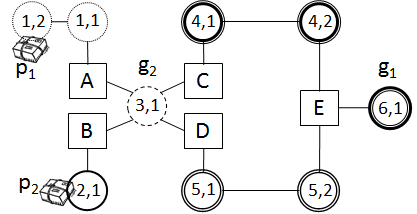
\includegraphics[scale=0.7]{Logistics}
\label{fig:logistics}
%\caption{A logistics example, where trucks deliver packages between logistics centers, denoted by squares. Each agent covers a set of cities, denoted by circles, and labeled $i,j$ where $i$ is the agent covering the city and $j$ is the local city index. The logistic centers can be entered by several agents, serving as collaboration sites.}
\caption{A logistics example.}
\end{figure}


Research on privacy preserving planning focuses on variants of the multi-agent STRIPS model (MA-STRIPS)~\cite{brafman2013complexity} mainly due to its simplicity. 
%We use here a multi-valued variables variant introduced recently by Brafman~\cite{Brafman15}.

%%%% STANDARD MV-MA-STRIPS definition %%%%%%%%%%%%
\begin{definition}[MA-STRIPS]
An MA-STRIPS problem is represented by a tuple $\langle V, \{A_i\}_{i=1}^k, I ,G \rangle$ where:
\begin{itemize}
	\item $k$ is the number of agents
%	\item $V$ is a finite set of finite-domain variables. 
	\item $P$ is a finite set of facts (can be true of false). 
%    \item For $1\leq i \leq k$, $A_i$ is the set of actions agent $i$ can perform. 
    \item $A_i$ is the set of actions agent $i$ can perform. 
	\item $I$ is the start state.
	\item $G$ is the goal condition.	
\end{itemize} 
\label{def:ma-strips}
\end{definition}
%The domain of a variable $v\in V$ is denoted by $dom(v)$. 
%Each action $a=\langle pre,eff,c\rangle\in A=\cup_{i=1}^k A_i$ is given by its preconditions ($pre$), effects ($eff$), and cost ($c$). 
Each action $a=\langle pre(a), eff(a), c(a) \rangle$ is defined by its preconditions ($pre(a)$), effects ($eff(a)$), and cost ($c(a)$). Preconditions and effects are logical formulas of $P$. A state is a conjunction of facts (true or false). The goal $G$ is a also a conjunction of facts. The result of applying an action $a$ to a state $s$ is denoted by $a(s)$. A solution to a planning task is a {\em plan} $\pi=(a_1,\ldots,a_k)$ such that $G\subseteq a_k(\ldots(a_1(I)\ldots)$, i.e., a sequence of actions that transforms the initial state ($I$) to a state satisfying the goal condition ($G$). 

%Preconditions and effects are partial assignments to of values to variables in $V$. A state is a complete assignment to all variables in $V$ and the goal condition $G$ is a full or a partial assignment of values to variables in $V$. The result of applying an action $a$ to a state $s$ is denoted by $a(s)$. A solution to a planning task is a {\em plan} $\pi=(a_1,\ldots,a_k)$ such that $G\subseteq a_k(\ldots(a_1(I)\ldots)$, i.e., it is a sequence of actions that transforms the initial state ($I$) to a state that satisfies the goal condition ($G$). 


Figure~\ref{fig:logistics} illustrates a simple logistic example in which the agents are trucks tasked with delivering packages. %The variables $V=\{p1\_at, p2\_at, t1\_at, t2\_at, t3\_at, t4\_at, t5\_at, t6\_at \}$, 
The set of facts $P$ represent the location of the two packages and six trucks. Each truck has three actions: move, load, and unload, corresponding to moving the truck between locations, loading a package and unloading it. Trucks can only drive along the edges in Figure~\ref{fig:logistics}. Agents are heterogeneous  and their range is restricted, such that location $i,j$ can only be reached using truck $i$. The rectangles are logistic centers visited by multiple trucks that load or unload packages. 

\subsection{Privacy}

Privacy-preserving MA-STRIPS extends MA-STRIPS by defining sets of variables and actions as private, known only to a single agent. To define this notion of privacy more generally, let $public(P)$ and $public(A)$ be the set of public variables in $P$ and public actions in $A$, respectively. Similarly, $private_i(P)$ and $private_i(A)$ denotes the variables and actions that are private to agent $i$, respectively. For ease of exposition we assume that all goals are public, although our method can be extended to handle private goals.

A solution to a privacy-preserving MA problem, is a sequence of public and private actions. We say that the sequence of public actions in such a solution is a high-level, or public, plan, that must be extended to a full plan using private actions of various agents. Given a valid high-level plan each agent can plan independently to achieve the preconditions on the public actions it executes in the high level plan \cite{maliah2014privacyPreserving}.

% Local view of a public action
Consider a public action $a$ of agent $j$ from the perspective of agent $i$. 
The action is public, so agent $i$ knows about $a$'s existence. However, if $a$ has private preconditions and effects, they are only known to agent $j$ and are hidden from agent $i$. Formally, we define the {\em local view} of action $a=\langle pre(a),eff(a),c(a) \rangle$ by agent $i$, denoted $\pi_i(a)$, as 
\[ \pi_i(a)=\langle public(P)\cap pre(a), public(P)\cap eff(a), c(a) \rangle \]
$\pi_i(a)=a$ if $a$ is an action of agent $i$. 



\begin{definition}[Local View]
The {\em local view} of agent $i$ of an MA-STRIPS problem $\pi=\langle  P, \{A_i\}_{i=1}^k, I ,G \rangle$
is defined by the tuple 
$\pi_i=\langle
\pi_i(P), \{\pi_i(A_j)\}_{j=1}^k,\pi(I),\pi(G)
\rangle
$
where:
\begin{itemize}
\item $\pi_i(P)=public(P)\cup private_i(P)$
\item $\pi_i(I)=I \cap \pi_i(P)$
\item $\pi_i(G)=G \cap \pi_i(P)$
\end{itemize}
\label{def:local-view}
\end{definition}



In our running logistic example, assume now that each truck is owned by a different company, such that a truck from one company do not want to share its location and coverage (which locations it can drive to) with the other companies. Thus, all the facts representing the location of trucks are private, while the facts representing whether a package is at a logistic center are public. Only the load/unload actions at the logistic centers are public, where the move actions are private for each agent.  The local view of agent 3 consists of the facts representing package locations, the facts representing locations of truck $3$, the move actions of truck $3$, and the load/unload action of all agents. For example, the local view of a load action of another agent has a precondition regarding the location of the package only, ignoring the private precondition of the location of the truck. 





\begin{definition}[Privacy-Preserving MA-STRIPS]
A privacy-preserving MA-STRIPS problem is defined by an MA-STRIPS problem 
and the $public(\cdot)$ and $private_i(\cdot)$ functions for every $i\in[1,n]$. The task is to find a solution without revealing private information during planning. 
\label{def:private-ma-strips}
\end{definition}
 

It is unclear what constitutes as ``revealing private information''. Weak forms of privacy preserving consider a private information revealed only if it is explicitly communicated to another agent. For example, if a truck publishes to another agent its current location. 
Most research on privacy preserving planning maintain this weak form of privacy. However, recent work \cite{Brafman15} also considered a stronger form of privacy preserving in which private information cannot be inferred by an adversary agent. 

% What kind of privacy we are looking for
\subsubsection{Cardinality-Hiding Privacy}

%In this paper we suggest a degree of privacy that we refer to as {\em cardinality-hiding privacy}. Achieving this privacy requirement means that an adversary agent listening to the communication between the agents during planning and execution cannot infer the number of private variables or the size of their domain. Alternatively, given a PDDL multi-agent domain definition \cite{vstolba2015competition}, one can define privacy over objects, and hide the cardinality of the number of objects of a given type, such as cities or trucks.

We suggest a degree of privacy that we refer to as {\em cardinality-hiding privacy}. Achieving this privacy requirement means that an adversary agent listening to the communication between the agents during planning and execution cannot infer the number of private facts. Alternatively, given a PDDL multi-agent domain definition \cite{vstolba2015competition}, one can define privacy over objects, and hide the cardinality of the number of objects of a given type, such as cities or trucks.


Consider for example the logistic problem above. A privacy-preserving algorithm that achieves cardinality-hiding privacy is guaranteed to hide the number of private locations that each truck can reach, even if it is aware that agents control trucks that drive between locations.

It would be even more compelling, when agents control multiple trucks, to hide the number of trucks controlled by each agent. However, in the current definition of the problem, agents publish the load and unload actions as public. If {\em (load p t x)} is a public action that loads package $p$ from location $x$ onto truck $t$, then some information over the number of trucks is exposed by the public actions. For example, exposing 3 different public actions {\em load p1 t1 A}, {\em load p1 t2 A}, {\em load p1 t3 A}, loading the same package $p1$ at the same location $A$, reveals that the exposing agent controls at least 3 different trucks. Hence facts that participate in preconditions or effects of public actions cannot be completely hidden from other agents. On the other hand, 
the public actions do not reveal the number of private locations as drive actions between private locations are private, and are not published to the other agents. 


To show that an algorithm is cardinality-hiding privacy preserving, one can observe the communication between agents throughout the planning process. If the communication is identical whether the number of private facts of that agent is $0$ or $n$, then we can say that the algorithm is cardinality-hiding privacy preserving. Later in this paper we prove this property for our projection method. 

%For example, in our approach each agent publishes to the other agents a projection of its view of the world. In the logistic domain, the projection is identical whether the agent travels between 5 or 10 private locations. The privacy preserving algorithm described in this work hence achieves cardinality-hiding privacy. \roni{This has nothing to do with our approach: it is how the domain is constructed. I moved the gist of this above}



\section{Classical Projections and Regression}

We now discuss projections of a multi-agent problem into classical planning, and the regression of formulas through action sequences, both of which are key concepts in our projection algorithm.

\subsection{Classical Projections}


% What is a single-agent projection and a complete single agent projection
A {\em classical projection} of a multi-agent problem is a compilation of the problem into a classical single-agent problem. For example, one can consider the local view (Definition~\ref{def:local-view}) of the agent as a classical planning problem, pretending that the agent controls the public actions of other agents as well.

A classical projection is sound if the sequence of public actions in any solution to the projected problem, can be extended using private actions only to a full solution to the original multi-agent problem.

We say that a classical projection is {\em complete} if given a solution to the original MA-STRIPS problem, there exists a solution to the projected planning problem with the same sequence of public actions. An example of a complete classical projection is the local view projection. 

% Why complete single-agent projection is helpful
A complete classical projection can therefore at least provide a heuristic for solving the original problem \cite{nissim2014distributed}. Moreover, in many cases it provides a high level plan that can be extended by the private actions of individual agents to a complete solution.

%For example, one can consider the local view of the agent as a single agent problem, assuming that the agent controls the public actions of other agents as well.

%A helpful property of the local projection for agent $i$ is that it is complete, in that any solution to the MA-STRIPS problem must be a solution to the local projected problem. Thus, solving a local projection provides at least a heuristic for solving the original problem \cite{raz}, and in many cases it provides a skeleton of a solution that can be extended by the individual agents to a complete solution. 



% Limitations of a local view projection
\subsubsection{Dependencies}

While a local view of an agent is a complete single-agent projection, it fails to consider some dependencies between public actions of another agent. In particular, 
the local view of agent $i$ contains no information about {\em private dependencies} between public actions of agent $j$. These are dependencies caused by one action requiring a private fact as a precondition and the other action has this precondition as an effect. 

For example, the projection of the {\em (unload p t A)} action, which has private preconditions {\em (at t A)} and {\em (on p t)}, has no precondition in the local view. Agents may believe that unloading a package at arbitrary public locations is always possible. In this work we present a different projection where information about private dependencies is shared. This projection is based on the concept of {\em regression}. %, described below. 


%\roni{Add a connecting line}


%However, this projection is clearly very partial, as it fails to consider any private dependencies between public actions of other agents. For example, the projection of the {\em unload p t A} action, which has private preconditions {\em (at t A)} and {\em (on p t)}, has no precondition in the projection. Agents may hence believe that unloading a package at arbitrary locations is always possible.
%\item Thus, projections have been used ads a heuristic


\subsection{Regression}
% Intuition of what is a regression
Regression is a fundamental tool in automated planning, in which we ask what are the conditions needed to reach a state, or achieve a fact, or perform an action. More generally, if a formula $\phi$ describes a constraint on state facts and $a$ is an action then the regression of $\phi$ through $a$, denoted $rg_a(\phi)$, is a formula that describes the minimal constraints on state facts such that if we apply $a$ to a state that satisfies $rg_a(\phi)$ we will reach a state  that satisfies $\phi$. 


% Formal
In the context of classical planning, Rintanen \shortcite{Rintanen} describes how to compute the regression of a formula $\phi$ through an action $a$. We now review these definitions.  


For simplicity, we assume here that both the effect and the precondition of an action are conjunctions of literals. That is, we do not allow conditional effects or disjunction of preconditions. We assume that the initial state is induced by an $init$ action, which assigns to all predicates their value at the initial state of the problem. We also assume that both the preconditions and effects of all actions are consistent, e.g., for a given literal $l$, no effect or precondition contains both $l$ and $\neg l$. We use this restricted representation for ease of exposition only. We could also use Rintanen's full regression definition at the cost of a more complicated exposition. %explanation of our methods.

In this restricted representation, Rintanen's regression of a formula $\phi$ through an action $a$, defined only over a single literal or a conjunction of literals, is simplified as follows: %\roni{Why ``simplified''?} \guy{Because the original Rintanen definition with conditional effects is much more complex}:
\begin{align}
&rg_a(l)=  pre(a)  :  l \in eff(a)&\\
&rg_a(l)= false   :  \exists l' \in eff(a) \mbox{ s.t. } l,l' \mbox{ are mutex}&\\
&rg_a(l)= l  :  l,\neg l \not\in eff(a)&\\
&rg_a(\phi)=  \bigwedge_{l \in \phi} rg_a(l)  :  \phi = l_1 \wedge l_2 \wedge ... \wedge l_k &
\end{align}
The equation (2) states that the regression of a literal through an action that has conflicting effects with that literal is forbidden. A special case of this is when $a$ has $\neg l$ as an effect. Rintanen shows that if $s \models rg_a(\phi)$ then $a(s)$ satisfies $\phi$. 

In some cases the regression formula can become inconsistent. For example, a conjunction containing both $l$ and $\neg l$. Furthermore, given a mutex detection mechanism, we can identify a conjunction containing both $l_1$ and $l_2$ when $l_1$ and $l_2$ are known to be mutex. In such cases, we say that the formula is simplified to $false$. 

% A regression tree
We further define the regression tree of a conjunction formula $\phi$, denoted $T_{rg}(\phi)$. The nodes of the tree are labeled by formulas (given our restricted action definition, these formulas are only conjunctions of literals), and the edges are labeled by actions. We denote the formula associated with node $n$ by $n.\phi$. The set of outgoing edges of a node $n$ are labeled by all actions $a \in A$, s.t. $\exists l \in n.\phi : l \in eff(a)$. That is, all actions that provide at least one literal in $n.\phi$. %\roni{I suggest to explain it from the ingoing edges prespective, because  the top down process explained below needs the discover ingoing eges and not outgoing.}\guy{I don't understand this comment.}\roni{I mixed in and out going. Please ignore.}

The tree is constructed top down, starting from the root. Leaves are labeled by either $true$ or $false$. Every sequence of edges in every path from a $true$ leaf to the root in the regression tree corresponds to a plan that achieves $\phi$ --- the formula at the root of the tree. During the construction of the tree, we may reach a node $n'$ labeled by a formula $\phi'$ such that there exists an ancestor node $n$ of $n'$, labeled by a formula $\psi$, such that $\phi' \models \psi$. This means a cycle has been identified in the regression tree, and we need not further develop $n'$. To remove the cycle, we replace $\phi'$ with $false$. 





%\section{Solution Approach}
%\begin{itemize}
%\item Following the GPPP approach: plan public actions/effects, then ground them
%\item Compiling the 
%\item Levels of privacy
%\end{itemize}

%\section{Strong Projection using Inter-Action Dependencies}%Compiling Away Private Facts and Actions}
\section{Dependency-Preserving Projection}

We now present our novel projection that transforms a privacy-preserving MA-STRIPS problem into a single agent planning problem. This projection, which we call the {\em dependency-preserving projection} (DP projection), is unique in that it contains information about private dependencies while preserving cardinality hiding privacy. 


Intuitively, DP projection captures the private relationships between public actions of an agent $i$, that is, which public actions of $i$ should be executed to enable other public actions of $i$. The public dependencies through the public facts are maintained in the projection. We now explain in detail the construction of the projection.

The DP projection contains all the public facts of the multi-agent problem. For each public action $a$ of agent $i$, the projection contains a set of actions $\alpha(a)$, each representing a sequence of public and private actions taken prior to executing $a$,
and a set of dependency facts $\delta(a)$, representing the dependency of $a$ on the public actions in these sequences. 
Note that no private action or fact exists in this projection. 
%The private actions and facts of the agents do not exist in the projection. 


\subsection{Creating the Regression Tree}


% We run regression on the local planning problem (as define by the PSM guys)
Given a public action $a$ of agent $i$, we use regression to identify sequences of private and public actions of $i$, as well as public actions of other agents, that enable the agent to execute $a$. We construct a regression tree for $pre(a)$ over a slightly revised local view of agent $i$.



Instead of using the exiting public actions in the regression tree creation, we replace each public action with a revised version, that has no preconditions. Thus, we do not model the conditions required for the execution of pubic actions other than $a$, but rather how these public actions help us to execute $a$.  Specifically, let $a_p$ be a public action of agent $i$, or a local view of a public action of another agent. The revised action $a^r_p$ of $a_p$ is defined as:
\begin{eqnarray}
&pre(a^r_p)=true&\\
&eff(a^r_p)=\displaystyle\bigwedge_{l \in eff(a_p)}l \bigwedge_{l' \in pre(a_p), \neg l' \not\in eff(a_p)}l'&
\end{eqnarray}
That is, the effect of $a^r_p$ contains all the effects of $a_p$, as well as all preconditions of $a_p$ that are not removed by the effect of $a_p$. These effects model the state of the world after $a_p$ has been executed. As $a_p$ was executed, all its preconditions that were not deleted still hold. 

Every agent $i$ constructs, for every public action $a$, regression trees $T_{rg}(pre(a))$, using its private actions, and the revised version of the public actions of $i$ as well as the revisions of the local view of the public actions of other agents. The branches of the tree ending at leaves labeled by $true$ represent plans to achieve the precondition of $a$, assuming that other public actions can always be executed. 



\begin{figure}
\centering
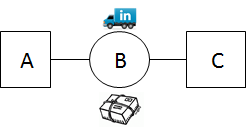
\includegraphics[scale=0.7]{SmallLogistics}
%\caption{A smaller logistics example domain of a single agent. Locations $A$ and $C$ are logistics centers, and $B$ is a private city. A truck $t$ and a package $p$ are initially at $B$.}
\caption{A simple logistics example.}
\label{fig:small}
\vspace{-0.3cm}
\end{figure}


\begin{figure}
\centering
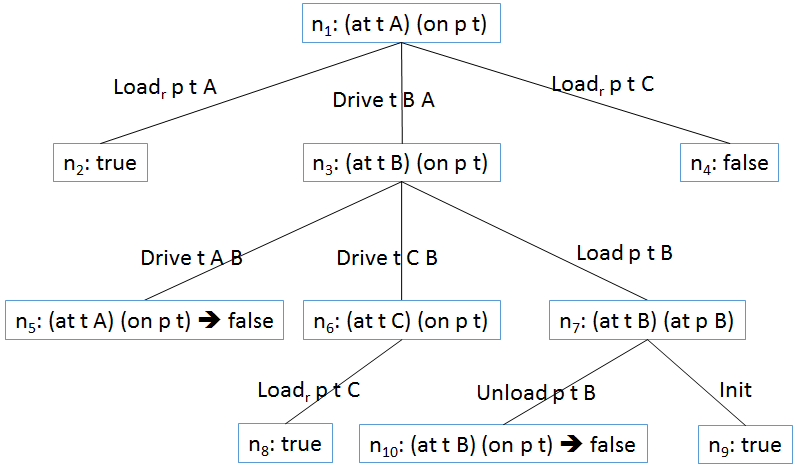
\includegraphics[scale=0.4]{RegressionTree}
\label{fig:tree}
\caption{Partial regression tree for {\em unload p t A} in Fig.~\ref{fig:small}.}
\vspace{-0.3cm}
\end{figure}


%\begin{example}
%\label{ex1}
Let us look at the smaller logistics example in Figure~\ref{fig:small}, where an agent has one private city $B$ and two public logistic centers $A$ and $C$. Figure~\ref{fig:tree} shows the regression tree constructed for  action {\em (unload p t A)} with precondition {\em(at t A)} and {\em(on p t)}. %Recalling that the revised action $load_r$ for the public {\em load p t A} action has the precondition $true$ and effect {\em (on p t) (at t A)}, we can see that
Since the revised action $load_r$ for the public {\em load p t A} action has the precondition $true$ and effect {\em (on p t) (at t A)}, regressing through this action results in the $true$ formula at node $n_2$. On the other hand, due to the conflict between {\em (at t A)} and the effect {\em (at t C)} of the revised action for {\em load p t C}, the regression result is $false$ for node $n_4$.

$n_5.\Phi$ is already satisfied by the formula at $n_1$, and is hence replaced by $false$, denoting a cycle. The same holds for $n_{10}.\phi$, satisfied by $n_3.\phi$. The $true$ leaves of the tree correspond to the plans {\em [load p t C, drive t C B, Drive t B A]},  {\em [init, load p t B, Drive t B A]}, and {\em [load p t A]}. 
%\end{example}

\subsection{Creating Projected Actions}

Given the regression trees $T_{rg}(pre(a))$, constructed to identify plans that achieve the precondition of a public action $a$ of agent $i$, we now define $\alpha(a)$ --- the set of projected actions corresponding to $a$, and $\delta(a)$ the set of dependency facts capturing the dependency of $a$ on the execution of other public actions of $i$. 

A projected action $a_{\{a_1,...,a_k\}}\in \alpha(a)$ represents the execution of $a$ after the public actions $a_1,...,a_k$ were already executed. A dependency fact $f^{a'}_a \in \delta(a)$ represents the dependency of $a$ on the execution of another public action $a'$.

We focus on public actions of agent $i$ that appear along some branch from a node labeled by $true$ to the root, supplying some private fact required for enabling a precondition of $a$. For each such public action $a'$, we introduce a new fact $f^{a'}_a \in \delta(a)$, representing the dependency of $a$ on the execution of $a'$. As $init$ may also appear along some branch, we can also have facts $f^{init}_a \in \delta(a)$, representing the dependency of $a$ on the initial state. 

Each branch $b$ from a leaf $n$ where $n.\phi=true$ to the root represents a plan for achieving $pre(a)$.
We are interested in the set of public actions $A_b$ that appear along the branch $b$ from a leaf $n$ to the root ($pre(a)$), achieving at least one private fact during the regression. The same set of public actions may appear in different branches of the tree, and we ignore such duplicates for privacy reasons. 

For each such set of actions $A_b$ we construct a projected action $a_b$ and add it into $\alpha(a)$. The precondition of $a_b$ contains the public preconditions of $a$, in conjunction with $\bigwedge_{a' \in A_b}f^{a'}_a$, representing that executing these public actions enables some private precondition of $a$. Let $\beta(a)$ be the dependency facts $f^a_{a'} \in \delta(a')$ over all $a'$, capturing the dependency of other actions $a'$ on $a$. The effect of every action in $\alpha(a)$ is the public effects of $a$, as well as $\bigwedge_{f \in \beta(a)} f$. 


\subsection{Removing Consumed Dependencies}


In many cases, the plan along a branch $b$ of the regression tree for $pre(a)$, or the action $a$ executed after the plan, may ruin some private effect $l$ of a public action $a'$ that appears in that branch. In that case, all other actions that rely on $a'$ can no longer depend on the effects of $a'$ to hold. Thus, when the execution of the plan that corresponds to $b$ removes a private effect of $a'$, we add to the effect of $a_b$ the conjunction $\bigwedge_{f \in \beta(a')} \neg f$, removing all the dependency facts that were achieved by executing $a'$. We denote the set of dependency facts deleted by an action $a_b$ by $delete(a_b)$.

Algorithm~\ref{alg:projection} describes the process of our DP projection of a single agent $i$ into a classical problem. The complete projection is the union of the  projections of all agents.



\begin{algorithm}[b!]
\small
	\SetKwBlock{Project}{Project($\pi_i$)}{end}
\Project{
	\KwIn{$\pi_i$, the local view of agent $i$}
    \KwOut{$\pi^p_i$, a projected classical planning problem}
    
	\ForEach{public action $a \in A_i$}{
		compute $T_{rg}(pre(a))$  \nllabel{line:proj:l1}\\
        compute $\delta(a), \beta(a)$\\
    }
	\ForEach{public action $a \in A_i$}{
\ForEach{branch $b$ in $T_{rg}(pre(a))$}{
			compute $a_b$: \\
			$pre(a_b) = pre(a) \displaystyle\bigwedge_{a' \in b}f^{a'}_a$  \\
        	$eff(a_p) = \displaystyle\bigwedge_{l \in eff(a) \cap public(P)}l 
        	\displaystyle\bigwedge_{\beta(a)} f^a_{a'} 
        	\displaystyle\bigwedge_{f^{a'}_{a''} \in delete(a_b)} \neg f^{a'}_{a''}$ \\
            add $a_b$ into $\alpha(a)$
        }
    }
	$\pi^p_i.A = \bigcup_{a \in public(i)} \alpha(a)$ \\
	$\pi^p_i.P = P \cup \{f^{a'}_a\}$ \\
    $\pi^p_i.G = G$ \\
    $\pi^p_i.I = I \cap P \cup \{f^{init}_a\}$\\
    \Return $\pi^p_i$   \\
}
\caption{Computing the DP projection for agent $i$} 
\label{alg:projection}
\end{algorithm}



%\begin{example}
In the previous example, given the public actions at the branches ending at the 3 $true$ leaves, we introduce dependency facts $f^{\tiny\mbox{{\em load p t A}}}_{\tiny\mbox{{\em unload p t A}}}$, $f^{\tiny\mbox{{\em load p t C}}}_{\tiny\mbox{{\em unload p t A}}}$, and $f^{\tiny\mbox{{\em init}}}_{\tiny\mbox{{\em unload p t A}}}$. We create 3 actions, corresponding to these branches. For example $a_{n_8}$, corresponding to the branch ending at node $n_8$, has precondition {\em $f^{\tiny\mbox{load p t C}}_{\tiny\mbox{unload p t A}}$}, because {\em load p t C} adds a private fact {\em (on p t)}. The effect of $a_{n_8}$ contains {\em (at p A)}, and deletes all facts $f^{\tiny\mbox{{\em load p t C}}}_a$ for all actions $a$, as it destroys the private effect {\em (on p t)} of the action {\em load p t C}.

%Observing the regression tree, it is easy to see that r
Replacing $B$ with a set of connected private locations $B_1,...,B_n$, would result in a different regression tree, but all the $true$ leaves in this tree would correspond to either the package at $A$ or $C$, or loading the package at its initial private location. Thus, the projection would be identical regardless of the number of private locations, preserving cardinality-hiding privacy.
%\end{example}


\begin{theorem}[DP Projection is Cardinality-Hiding]
An agent that receives a DP projection computed by a different agent 
cannot infer the cardinality of private facts. 
\label{the:dp-proof}
\end{theorem}
{\bf Proof outline:}
The DP projection relies on the dependency tree for each public action $a_p$ of agent $i$. Given a regression tree, one could add private facts (and private actions that manipulate them) that will not modify the number of $true$ leaves, or the sequence of public actions in each $true$ branch.
Moreover, we could add any number of private facts and private actions that would modify the number of leaves, yet each leaf in the new tree would contain the same set of public actions as a leaf in the original tree. In these cases, although the number of private facts and actions was modified, the projection  does not change. 




\subsection{Application of a DP Projection}
Consider the following effective application of DP projection in a planner. First, each agent computes a DP projection and broadcasts it to all agents. Following, an off-the-shelf classical planner finds a solution to the joint DP projection, resulting in a  high-level plan. Finally, each agent extends this high-level plan to be able to execute the public actions in it, again, using an off-the-shelf classical planner.  

At least theoretically, it is possible that the generated high-level plan cannot be extended. While in our experiments this never happened, it is possible, for completeness, to simply search for a new high-level plan by resuming the search for solutions of the DP projection. We call the resulting planner the {\em DP-projection planner}, or simply DPP.


%\section{Incomplete Compilation}
%\guy{I am in favor of removing this section, and adding a formal proof of cardinality privacy if possible}
%\begin{itemize}
%\item The compilation can be problematic because a complete regression may be exponential
%\item Solution: a GPPP-like approach, first finding a coordination scheme and then grounding
%\item Theoretical claims: proof of completeness and soundness.
%\end{itemize}



%\section{Coordinated Grounding}
%\guy{This should be removed - we don't have space and this is a complete orthogonal contribution - let's write a paper to ICAPS on various grounding methods}

\section{Experimental Results}

%To evaluate our approach we experiment with benchmarks from the recent CoDMAP competition \footnote{\url{http://agents.fel.cvut.cz/codmap/results/}}. We run our algorithm locally, on a 2.66 GHz machine with 24 cores and 32 GB of memory. Our projection approach solves the high level plan using both FF \cite{hoffmann2001ff} and FD \cite{helmert2009landmarks}. After the high level plan has been found each agent plans to achieve its own actions using FF. The results of other planners are taken from the recent rerun of the competition. \roni{This uses a ``high-level'' term that was not used so far.}
We experimented with benchmarks from the 2015 CoDMAP competition~\cite{vstolba2015competition}.\footnote{\url{http://agents.fel.cvut.cz/codmap/results/}} 
We run DPP on a 2.66 GHz machine with 24 cores and 32 GB of memory. DPP was implemented using both FF \cite{hoffmann2001ff} and FD \cite{helmert2009landmarks} for the high-level planning and FF for extending high-level plans.

%Our  approach first applies our strong projection and solves it using both FF \cite{hoffmann2001ff} and FD \cite{helmert2009landmarks} \roni{I think we should say what configuration of FD was used.}. Then, each agent plans to achieve the actions assigned to it in the projection solution by using FF. The results of other planners are taken from the recent rerun of the competition. 

%We compare DPP with the best performing and most relevant privacy-preserving planners: {\bf GPPP.}~\cite{maliah2015privacy} A joint search mechanism, using the privacy preserving landmark heuristic.  {\bf MAPlan/FF+DTG.} An extension of the MAFS algorithm~\cite{nissim2014distributed} using the FF and DTG heuristics together.  {\bf MAPR-p.} A planner that plans for each agent sequentially, where goals that were not achieved by one agent are assigned to the subsequent agents.  {\bf PRM.} The plan merging and replan (PMR) planner~\cite{luis2014planMerging}.  {\bf PSM-VRD.} The PSM planner~\cite{tovzivcka2014generating,jakubuv2015multiagent}, which constructs a finite state machine for the plans of each agent.

We compare DPP with the best performing and most relevant privacy-preserving planners: GPPP~\cite{maliah2015privacy}, MAPlan/FF+DTG (an extension of the MAFS algorithm~\cite{nissim2014distributed} using the FF and DTG heuristics together), MAPR-p, PMR~\cite{luis2014planMerging}, and PSM-VRD~\cite{tovzivcka2014generating,jakubuv2015multiagent}. Details on these planners can be found in the CoDMAP website.

Table~\ref{tbl:codmap} presents the number of instances solved under a 30 minutes timeout (also known as ``coverage'') over the domains in the competition. The results indicate that our projection approach -- DPP -- solves more problems than all other approaches. The most important difference between DPP and all other planners, is that we use, once the projection was constructed, an off-the-shelf classical planner, rather than a coordinated joint search mechanism. Our results point to the strengths of the mature classical planners over the rather new joint search mechanisms.

\begin{table}
\centering
\scriptsize
\begin{tabular}{l|rrrrrr}

Domain			&GPPP	&MAPR	&PMR	&MAPlan/ &PSM-	&DPP\\
	    		&		&-p	    &	    &FF+DTG	 &VRD	&\\\hline
blocksworld		&12		&20		&20		&20		&20		&20\\
depot			&11		&0		&0		&13		&17		&19\\
driverlog		&14		&20		&19		&17		&20		&20\\
elevators		&20		&19		&19		&11		&12		&17\\
logistics		&20		&19		&0		&18		&18		&20\\
rovers			&19		&19		&20		&20		&12		&20\\
satellites		&18		&20		&19		&20		&18		&20\\
sokoban			&9		&0		&6		&18		&18		&17\\
taxi			&20		&0		&19		&20		&0		&20\\
wireless		&3		&2		&7		&4		&0		&9\\
woodworking		&18		&0		&0		&16		&19		&19\\
zenotravel		&20		&20		&18		&20		&13		&20\\	\hline
sum				&184	&139	&147	&197	&167	&221\\

\end{tabular}
\caption{Coverage results for a timeout of 30 minutes over the CoDMAP instances.}
\label{tbl:codmap}
\vspace{-0.5cm}
\end{table}






\section{Discussion and Related Work}

A similar idea to our projection was suggested by the PSM planner~\cite{jakubuv2015multiagent}. In PSM each agent finds plans that solve the simple projection of the original problem, and then employ a mechanism to check if the plans generated by all agents are valid together. If not, the search continues. The agents publish plans as state machines, rather than sequences of actions. More recently, they even used {\em dependency graphs}~\cite{tozicka2015internally} to captures information similar to the regression trees we create. However, in their approach either the entire private dependency graph can be reduced to a single node, and thus can be published to the other agents or not. In many other benchmark domains, however, some private nodes remain and thus in such cases, no dependencies were published. Our approach is able to public partial dependencies in such cases.


%Another relevant approach by the same authors uses {\em dependency graphs}~\cite{tozicka2015internally}. A dependency graph is a graph whose nodes are either facts or actions, there is an edge from every fact to actions that use it as precondition, and an edge from every action to the facts in its effect. The dependency graph captures information that is very similar to the regression trees that we create.

%They combine together nodes in the dependency graph whenever joining these nodes does not affect the public information. In some domains, the entire private dependency graph can be reduced to a single node, and thus can be published to the other agents without compromising privacy. In many other benchmark domains, however, some private nodes remain, and publishing the resulting graph would still reveal private information. Therefore, in such cases, no dependencies were published.  

The completeness of our projection is compromised because our mechanism for consuming dependencies is too strong, removing in some cases dependencies that are still maintained. One can remove this mechanism to achieve completeness, resulting in a delete-relaxation formalization over the private facts. In our experiments, though, this resulted in unsound high level plans. % that could not be executed.
We conjecture that our projection is sound, but a soundness proof is still an open question. In our experiments, every high level plan produced by the projection was then verified to be sound.

%Assumptions made by Ext D planner:
%\begin{itemize}
%\item All precondition as action-consuming, i.e., if $f$ is a precondition then it is also in the delete effects.
%\item All delete effects are also preconditions, i.e,. if $f$ is a delete effect it is also a precondition. 
%\end{itemize}

%Notes:
%1. They also added a init action.\\
%2. Reduction rules:\\
%R1. Remove a chain (a1->f->a2->X, becomes just a12->X\\
%R2. Remove small cycles (a1->a2->a1) becomes just a1\\
%R3. Remove structurally equivalent nodes (if a1->f1->a2 and a1->f2-a2 then remove f1 or f2).\\
%R4. Remove orphan facts (facts that are not preconditions of any action).     

In the context of multi agent planning, several types of privacy were suggested in the past. Most notably, Brafman~\cite{Brafman15} defines weak privacy, where no private fact is explicitly sent to other agents, and strong privacy, where agents cannot infer any private information from the communication during the plan computation.

While strong privacy is certainly desirable, there is currently no known algorithm that preserves strong privacy for a reasonable set of benchmarks. Specifically, Brafman demonstrated that a variant of MAFS, called SECURE-MAFS, maintains strong privacy only for a version of logistics, where every location under the responsibility of an agent is reachable from any other location without passing through a public location, and for domains such as satellites, where all agents can achieve all goals independently without collaboration, and the plan only assigns tasks to agents.

Furthermore, Brafman requires that the heuristic that is used during plan search relies only on the public information, as can be done using the local view projection of the problem. More informed heuristics, such as Landmarks\cite{maliah2014privacyPreserving,vstolba2014relaxation} or the FF heuristic \cite{vstolba2015admissible}



\section{Conclusion}
In this paper we suggest a strong projection of a privacy preserving multi-agent problem onto a classical planning problem. We demonstrate that planning using this projection allows us to solve more benchmark problems than any other state-of-the-art privacy preserving planner. We also provide a new definition of privacy, showing our projection to conform to this new definition. Future work will investigate theoretical properties of our projection, as well as develop more sophisticated projections that able to preserve dependencies and completeness.



%Our current projection is incomplete, which is unfortunate. One interesting future research direction is in creating projections that are complete, while still preserving the action dependencies. It is also important to analyze other state-of-the-art planners with respect to our cardinality-hiding privacy definition.

\pagebreak
\bibliographystyle{aaai}
\bibliography{library}
\end{document}